% \chapter{N-Fold via LP rounding} \label{platform}
\newpage
\section{N-Fold via LP rounding}  % Set the left side page header

The main drawback of the augmentation algorithm is that after solving the linear relaxation, we can be arbitrarily far from the optimal solution of the IP, what means that we need many augmentation steps. In this section we follow another approach introduced in \cite{EISENBRAND:2020} based on a more restricted linear relaxation which optimum is closer to the optimum of the IP and we prove this. We then show how to take advantage of this proximity bound to obtain the current fastest algorithm for the N-Fold case, running in roughly linear time.


\subsection{Restricted linear relaxation}

Following the previous block decomposition of the variables in the N-Fold IP we can express the N-Fold IP as:
\begin{equation*}
    % TODO: Maybe call it IP_A(b,c)??
    (N-Fold IP) \equiv max\{\sum (c^{(i)})^t y^{(i)} : \sum A^{(i)} y^{(i)} = b_0, l_i \leq y^{(i)} \leq u_i, y^{(i)} \in P_i \}
\end{equation*}
\vspace{-50pt}
% TODO: Change this!
\begin{center}
$A \in \mathbb{Z}^{mxn}$, $b \in \mathbb{Z}^m$, $c \in \mathbb{Z}^n$, $l$  and $u$ lower and upper bounds for x
\end{center}

The main idea of the restricted linear relaxation is that we restrict each region $P_i$ to $Q_i = conv(P_i \cap \mathbb{Z}^t)$.

\begin{figure}[h]
\centering
\begin{minipage}[b]{0.45\textwidth}
    \centering
    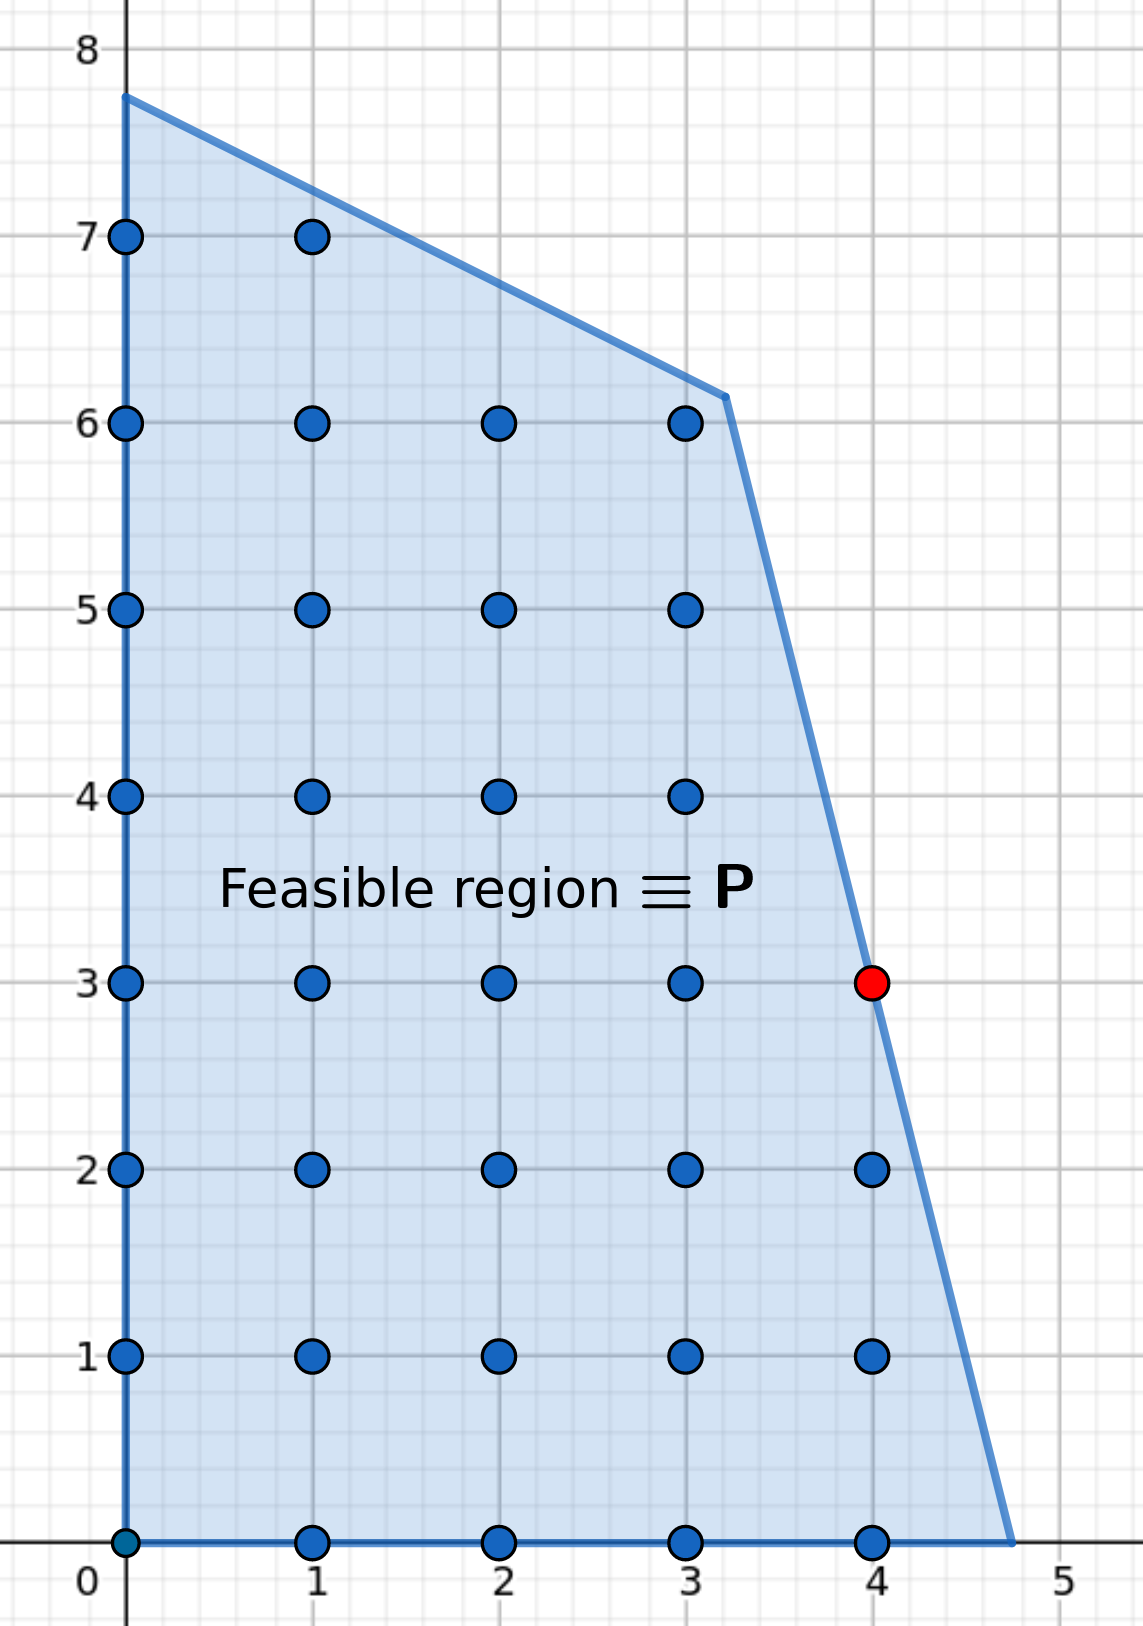
\includegraphics[width=0.9\textwidth]{images/IP(12).png}
    % TODO!
    \caption{Complete this}
\end{minipage}
\hfill
\begin{minipage}[b]{0.45\textwidth}
    \centering
    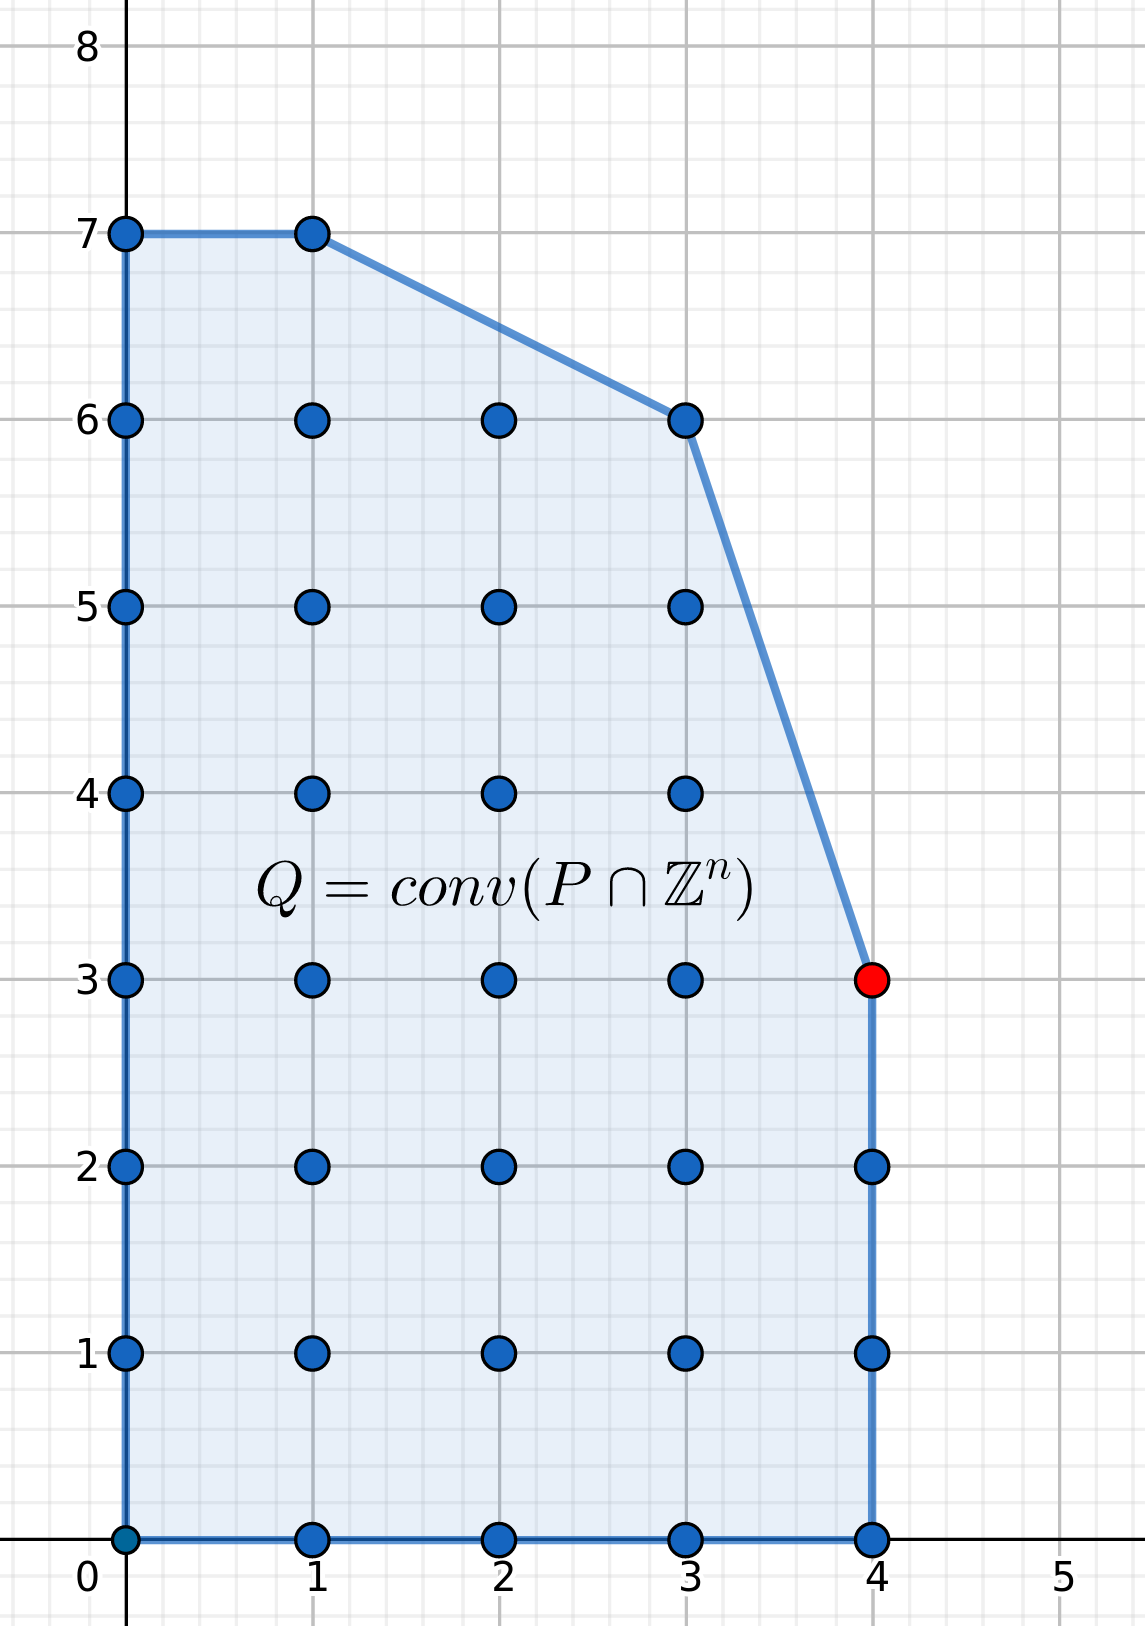
\includegraphics[width=0.9\textwidth]{images/IP(10).png}
    % TODO!
    \caption{Also this}
\end{minipage}
\end{figure}

% TODO: Ellipsoid method!!
Solving the restricted linear relaxation problem is not an easy task in practice at all but it was proved in \cite{EISENBRAND:2020} that it can be solved in linear time (ignoring logarithmic factors). 

% TODO: Not going deeper but references or really short explanation
\begin{proposition}[\textbf{N-Fold RLR complexity}]
    The N-Fold IP restricted linear relaxation problem can be solved in time
    \begin{equation*}
        O(nt \cdot log^2(nt) \cdot \varphi p(r) (s\Delta)^{O(s^2)})
    \end{equation*}
\end{proposition}

% TODO: The solution of the RLR hasn't to be integer
% TODO: But it verifies some properties which end in this lemma!
\begin{proposition}[\textbf{N-Fold proximity to RLR}]
    Let $x^*$ be an optimal vertex solution of a N-Fold RLR, then there exists an optimal solution $z^*$ for the N-Fold IP verifying:  
    \begin{equation*}
        ||z^* - x^*||_1 \leq (rs\Delta)^{O(rs)}
    \end{equation*}
\end{proposition}
\hspace{15pt}[Cslovjecsek, Eisenbrand, Weismantel 2020]

\newpage
\subsection{Dynamic program}        

We present in this section a dynamic program which takes us from an optimal solution to the restricted linear relaxation to the optimal solution of the N-Fold IP.

% TODO: Proof? At least explanation or references
\begin{proposition}[\textbf{N-Fold RLR to optimum complexity}]
    Given an optimal vertex of an N-Fold RLR, the N-Fold IP can be solved in time
    \begin{equation*}
        O(nt \cdot (rs\Delta)^{O(r^2s+s^2)})
    \end{equation*}
\end{proposition}
%\hspace{15pt}[Cslovjecsek, Eisenbrand, Weismantel 2020]
\begin{proof}

    
We now define the set $S_\ell$ as the set of $y \in \mathbb{Z}^r$ such that:
\begin{equation*}
\sum_{i=1}^\ell A_ix_i^* - \gamma \leq y \leq \sum_{i=1}^\ell A_ix_i^* + \gamma 
\end{equation*}
        
        
We can construct a weighted directed acyclic graph G(V,E) with vertices:
\begin{equation*}
    V = \{(\ell,y) / y \in S_\ell\} \cup \{ (0,0), (n,b_0) \}
\end{equation*}
        
Weighted edges between $(\ell-1,y)$ and $(\ell,y')$ if the problem is feasible:
        
\begin{equation*}
    max\{c_\ell^tx: A_\ell x = (y'-y), B_\ell x = b_\ell, l_\ell \leq x \leq u_\ell \}
\end{equation*}
        
A longest path from $(0,0)$ to $(n,b_0)$ in G(V,E) corresponds to an optimal solution of the N-Fold integer program.

% PART 1: Point z => Path (and path cost >= c^t z)
Let $\gamma := (rs\Delta)^{O(rs)}$. For every $1 \leq \ell \leq n$:
% TODO: Switch to equation* maybe!
\begin{align*}
    ||x^* - z||_1 \leq \gamma 
    & \implies \sum_{i=1}^\ell ||x_i^* - z_i||_1 \leq \gamma\\ 
    & \implies \sum_{i=1}^\ell ||A_i(x_i^* - z_i)||_\infty \leq \Delta \gamma = \gamma
\end{align*}

% TODO: The proximity bound ensures that at least one optimum is here! 
Therefore, for every feasible point z verifying the proximity bound we have:
\begin{equation*}
    % \forall 1 \leq l \leq n
    \sum_{i=1}^\ell A_ix_i^* - \gamma \leq \sum_{i=1}^\ell A_iz_i \leq \sum_{i=1}^\ell A_ix_i^* + \gamma 
    %& \leq s\Delta \sum_{i=0}^l ||x^* - z^*||_\infty \\
    %& \leq s\Delta \sum_{i=0}^n ||x^* - z^*||_\infty \\
    %& \leq s\Delta (rs\Delta)^{O(rs)} = (rs\Delta)^{O(rs)}
\end{equation*}

Graph plot for the proof of algorithm complexity:
------------------------------------------------------
    \begin{center}
    \begin{tikzpicture}[
            > = stealth, % arrow head style
            shorten > = 1pt, % don't touch arrow head to node
            auto,
            node distance = 3cm, % distance between nodes
            semithick % line style
        ]

        \tikzstyle{every state}=[
            draw = black,
            thick,
            fill = white,
            minimum size = 4mm
        ]

        \node[state, minimum size=0.8cm] (s) at (0,0) {$0$};
        
        %\node[state] (w1) at (2,2)  {$y_{11}$};
        %\node[state] (u1) at (2,0)  {$y_{12}$};
        \node (v1) at (2,-2) {$A_1z_1$};
        
        %\node (u2) at (4,0)  {$\sum_{i=1}^\ell A_ix^*$};
        \node (w2) at (4,2)  {$\sum_{i=1}^2A_iz_i$};
        %\node[state] (u2) at (4,0)  {$y_{22}$};
        %\node[state] (v2) at (4,-2) {$y_{23}$};
        
        %\node[state] (w3) at (6,2)  {$y_{31}$};
        \node (u3) at (6,0)  {$\sum_{i=1}^3A_iz_i$};
        %\node[state] (v3) at (6,-2) {$y_{33}$};
        
        \node (w4) at (8,2)  {$\sum_{i=1}^4A_iz_i$};
        %\node[state] (u4) at (8,0)  {$y_{42}$};
        %\node[state] (v4) at (8,-2) {$y_{43}$};
        
        \node (f) at (10,0)  {$\sum_{i=1}^nA_iz_i = b_0$};
        
        \path[->] (s) edge node  {$\geq c_1^tz_1$} (v1);
        \path[->] (v1) edge node {$\geq c_2^tz_2$} (w2);
        \path[->] (w2) edge[below left] node {$\geq c_3^tz_3$} (u3);
        \path[->] (u3) edge node {$\geq c_4^tz_4$} (w4);
        \path[->] (w4) edge node {$\geq c_5^tz_5$} (f);

        \draw[red, dashed] (1, 3) -- (1, -3);
        \draw[red, dashed] (3, 3) -- (3, -3);
        \draw[red, dashed] (5, 3) -- (5, -3);
        \draw[red, dashed] (7, 3) -- (7, -3);
        \draw[red, dashed] (9, 3) -- (9, -3);
        
        % \node (S1) at (2,-3.5) {$S_1$};
        % \node (S2) at (4,-3.5) {$S_2$};
        % \node (S3) at (6,-3.5) {$S_3$};
        % \node (S4) at (8,-3.5) {$S_4$};
    \end{tikzpicture}
    \end{center}


What this means is that we have vertices in $S_\ell$ (mention explicitly!) and edges (thanks that the problem has a feasible point given by the next element of the partial sum). Note also that these feasible point is of course lower or equal than the optimal solution of this edge problem and therefore the path has cost greater or equal than the objective function in that point.

% PART 2: Path (and path cost C) => Point (and objective function value C)

Analogously if we have a path from $0$ to $b_0$ we have vertices and edges. The edges are associated with optimal solutions for the edge IP and thanks to start in 0 and finishing in $b_0$ we can construct a feasible point since this optimal solutions for the edges problem. Also the path cost is the value of the objective function in this point so every path is associated with a feasible point and it's cost is bounded by the optimal solution of the IP.


\begin{center}
\begin{tikzpicture}[
        > = stealth, % arrow head style
        shorten > = 1pt, % don't touch arrow head to node
        auto,
        node distance = 3cm, % distance between nodes
        semithick % line style
    ]

    \tikzstyle{every state}=[
        draw = black,
        thick,
        fill = white,
        minimum size = 4mm
    ]

    \node[state, minimum size=0.8cm] (s) at (0,0) {$0$};
    
    %\node[state] (w1) at (2,2)  {$y_{11}$};
    %\node[state] (u1) at (2,0)  {$y_{12}$};
    \node[state] (v1) at (2,-2) {$y_{13}$};
    
    %\node (u2) at (4,0)  {$\sum_{i=1}^\ell A_ix^*$};
    \node[state] (w2) at (4,2)  {$y_{21}$};
    %\node[state] (u2) at (4,0)  {$y_{22}$};
    %\node[state] (v2) at (4,-2) {$y_{23}$};
    
    %\node[state] (w3) at (6,2)  {$y_{31}$};
    \node[state] (u3) at (6,0)  {$y_{32}$};
    %\node[state] (v3) at (6,-2) {$y_{33}$};
    
    \node[state] (w4) at (8,2)  {$y_{41}$};
    %\node[state] (u4) at (8,0)  {$y_{42}$};
    %\node[state] (v4) at (8,-2) {$y_{43}$};
    
    \node[state, minimum size=0.8cm] (f) at (10,0)  {$b_0$};
    
    \path[->] (s) edge node  {$c_1^tu_1^*$} (v1);
    \path[->] (v1) edge node {$c_2^tu_2^*$} (w2);
    \path[->] (w2) edge node {$c_3^tu_3^*$} (u3);
    \path[->] (u3) edge node {$c_4^tu_4^*$} (w4);
    \path[->] (w4) edge node {$c_5^tu_5^*$} (f);

    \draw[red, dashed] (1, 3) -- (1, -3);
    \draw[red, dashed] (3, 3) -- (3, -3);
    \draw[red, dashed] (5, 3) -- (5, -3);
    \draw[red, dashed] (7, 3) -- (7, -3);
    \draw[red, dashed] (9, 3) -- (9, -3);
    
    % \node (S1) at (2,-3.5) {$S_1$};
    % \node (S2) at (4,-3.5) {$S_2$};
    % \node (S3) at (6,-3.5) {$S_3$};
    % \node (S4) at (8,-3.5) {$S_4$};
\end{tikzpicture}
\end{center}

\end{proof}

\textbf{Facts for N-Fold complexity}
\begin{itemize}
    \item $|S_l| \leq (rs\Delta)^{O(r^2s)}$
    \item $|V| + |E| \leq O(n(rs\Delta)^{O(r^2s)})$
    \item The edge IP can be computed in time $t((r + s)\Delta)^{O(r + s)^2}$
    \item Longest path problem in a acyclic digraph can be solved in linear time.
\end{itemize}

\textbf{N-Fold complexity}
\begin{itemize}
\item \textbf{N-Fold complexity}\\
    The N-Fold IP can be solved in time $nt(rs\Delta)^{O(r^2s + s^2)} + RLR$
\end{itemize}
\hspace{15pt}[Cslovjecsek, Eisenbrand, Weismantel 2020]